\documentclass[conference]{IEEEtran}
\usepackage[utf8]{inputenc}
\usepackage[T1]{fontenc}
\usepackage{hyperref}
\usepackage{amsmath}
\usepackage{amssymb}
\usepackage{graphicx}
\usepackage{cite}
\bibliographystyle{IEEEtran}

\begin{document}

\title{Cross-Modal Attention Fusion for Anterior Segment Segmentation Using Complementary Image Representations}

\author{
    \IEEEauthorblockN{Caleb Alfaro}
    \IEEEauthorblockA{\textit{Computing Engineering}\\
    Instituto Tecnológico de Costa Rica\\
    calebam2112@gmail.com}
    \and
    \IEEEauthorblockN{Desireé Avilés}
    \IEEEauthorblockA{\textit{Computing Engineering}\\
    Instituto Tecnológico de Costa Rica\\
    desiree.aviles.a@gmail.com}
    \and
    \IEEEauthorblockN{Danilo Duque}
    \IEEEauthorblockA{\textit{Computing Engineering}\\
    Instituto Tecnológico de Costa Rica\\
    daniloduquedg@gmail.com}
}

\maketitle

\begin{abstract}
Accurate segmentation of anterior segment structures — including the cornea, pupil, and lens — is clinically relevant for cataract assessment and surgical planning. Unimodal approaches that operate solely on RGB images are sensitive to lighting artifacts and the low color contrast caused by lens opacification, limiting their reliability in real-world ophthalmic settings. We propose a dual-encoder architecture that fuses complementary representations of the same image to address this limitation. One encoder processes the original RGB image to capture photometric and textural features, while a parallel encoder processes a structural edge map derived via Canny filtering to capture geometric boundary information. A cross-attention module at the bottleneck allows the RGB encoder to query the edge encoder's feature space, enriching the primary representation with explicit structural cues before decoding. Although both inputs originate from the same image, they occupy heterogeneous feature spaces — photometric and geometric — qualifying the approach as multimodal fusion in the architectural sense. We evaluate the proposed model on the Cataract-Seg dataset against unimodal U-Net baselines and an early-fusion concatenation baseline, reporting Intersection over Union (IoU) and Dice coefficient as primary metrics. The proposed cross-attention fusion strategy demonstrates improved boundary delineation under variable imaging conditions, supporting its suitability for resource-constrained clinical deployments relative to large foundation model adaptations.
\end{abstract}

\begin{IEEEkeywords}
    cataract segmentation, cross-modal attention, anterior segment, deep learning, multimodal fusion
\end{IEEEkeywords}

\section{Introduction}
Your introduction goes here.

\section{Related Work}

\subsection{Anterior Segment and Cataract Segmentation}

Encoder-decoder architectures have become the dominant paradigm for medical image segmentation since Ronneberger et al.\ introduced U-Net \cite{ronneberger2015unet}, demonstrating that a contracting path paired with a symmetric expanding path enables precise localization from very few annotated images. This architecture has been widely adopted in ophthalmic segmentation due to its ability to preserve fine spatial detail through skip connections.

The nnU-Net framework \cite{isensee2021nnunet} extended this foundation by automatically configuring the network architecture, preprocessing, and training strategy for any given dataset. Its strong performance on 23 public benchmarks established it as a competitive baseline for medical segmentation tasks, including ophthalmic structures, without task-specific engineering.

Surgical scene understanding in cataract procedures presents additional challenges due to specular reflections, occlusions from instruments, and intraoperative illumination changes. The CaDIS dataset \cite{grammatikopoulou2021cadis} addressed this gap by providing richly annotated frames of cataract surgery videos covering anatomical structures and surgical instruments. Building on such data, Ghamsarian et al.\ proposed DeepPyram \cite{ghamsarian2022deeppyram}, a pyramid-view architecture with deformable receptive fields designed to handle the multi-scale structure variability inherent in cataract surgery segmentation. DeepPyram demonstrated that standard convolutions benefit from explicit multi-scale context, motivating our use of complementary structural representations to further enrich feature diversity.

\subsection{Multimodal Fusion in Medical Imaging}

The transformer architecture introduced by Vaswani et al.\ \cite{vaswani2017attention} established attention mechanisms as a principled way to model long-range dependencies and cross-sequence interactions. Its key insight --- that queries from one representation can attend to keys and values from another --- directly motivates the cross-modal fusion strategy we adopt at the bottleneck.

In the medical imaging domain, Zhang et al.\ proposed mmFormer \cite{zhang2022mmformer}, a multimodal medical transformer that handles incomplete modality sets for brain tumor segmentation. By distributing modality-specific encoders connected through intra- and inter-modal transformers, mmFormer demonstrated that cross-modal attention outperforms simple feature concatenation when input representations are structurally heterogeneous. Similarly, Zhang et al.\ \cite{zhang2024dattnet} introduced DATTNet, a dual-attention transformer that models spatial and channel dependencies simultaneously in a hybrid CNN-transformer framework, achieving state-of-the-art results on multi-modal medical segmentation benchmarks.

Li et al.\ proposed DECTNet \cite{li2024dectnet}, a dual-encoder architecture combining a convolutional branch with a Swin Transformer branch, fusing their complementary representations via a feature fusion decoder. This direct structural precedent confirms the effectiveness of parallel encoders with heterogeneous inductive biases for medical segmentation. In contrast to DECTNet, which fuses different network types processing the same modality, our approach fuses two encoders processing structurally distinct representations (photometric and geometric) of the same image.

The multi-modal ophthalmic AI survey by Wang et al.\ \cite{wang2024multimodal} reviewed deep learning across fundus photography, OCT, OCTA, and clinical metadata, explicitly identifying cross-modal feature fusion as an open research direction with clinical impact. This motivates our exploration of intra-image multimodal fusion for cataract segmentation specifically.

\subsection{Foundation Models for Ophthalmic Segmentation}

Recent advances in foundation models have shifted the landscape of medical image segmentation. Ma et al.\ introduced MedSAM \cite{ma2024medsam}, fine-tuning the Segment Anything Model (SAM) on over 1.5 million medical image-mask pairs across 10 imaging modalities. While MedSAM achieves strong generalization, its scale --- requiring 20 A100 GPUs for training --- makes it impractical for deployment on small ophthalmic datasets without substantial computational infrastructure.

The challenge of adapting large models to specialized scenes was addressed by Chen et al.\ with SAM-Adapter \cite{chen2023samadapter}, which introduces lightweight task-specific adapters to guide SAM toward domain-specific features such as camouflage and shadow. While adapter-based methods reduce fine-tuning cost, they still inherit the full SAM encoder and are optimized for scenarios with large pre-training data available.

In ophthalmology specifically, Zhou et al.\ introduced RETFound \cite{zhou2023retfound}, a masked autoencoder pre-trained on 1.6 million retinal images that generalizes across multiple ophthalmic disease detection tasks. Similarly, Qiu et al.\ proposed VisionFM \cite{qiu2024visionfm}, a multi-modal multi-task vision foundation model validated on eight ophthalmic image modalities for disease diagnosis, prognosis, and anatomical segmentation.

\subsection{Positioning of the Proposed Work}

The above literature reveals three complementary trends: (1) task-specific architectures like U-Net and its variants achieve strong segmentation performance but are sensitive to the information available in a single imaging modality; (2) cross-modal attention mechanisms effectively fuse heterogeneous representations but have not been applied to intra-image geometric decomposition in cataract segmentation; and (3) foundation models provide generalization at scale but are inaccessible for small, specialized datasets.

Our proposed architecture bridges the gap between (1) and (2): we adapt the dual-encoder, cross-attention paradigm demonstrated in mmFormer and DECTNet to a lightweight, purpose-built model where the two encoders process the original RGB image and its Canny edge map respectively. This design explicitly provides the decoder with complementary photometric and geometric features through a bottleneck cross-attention module, without requiring large-scale pre-training. Compared to foundation model adaptation (3), this approach is computationally accessible and directly optimized for the structural characteristics of cataract anterior segment images.


\section{Proposed Method}

\subsection{Overview}

We propose a dual-encoder segmentation architecture that fuses two complementary representations of the same input image: the original RGB image and a structural edge map derived from it via Canny filtering. Although both inputs originate from a single image, they occupy heterogeneous feature spaces --- photometric and geometric --- and are processed by independent encoders whose representations are fused through a cross-attention module at the bottleneck before decoding.

\subsection{Input Representations}

Given an input image $\mathbf{I} \in \mathbb{R}^{H \times W \times 3}$, two representations are constructed:

\textbf{RGB stream.} The original image is normalized to $[0, 1]$ and resized to $512 \times 512$.

\textbf{Edge stream.} A single-channel edge map $\mathbf{E} \in \mathbb{R}^{H \times W \times 1}$ is computed by applying Canny edge detection to the grayscale conversion of $\mathbf{I}$, with thresholds $t_1 = 50$ and $t_2 = 150$. The edge map is replicated to three channels before encoding. This representation makes explicit the geometric boundary structure that is clinically relevant for lens delineation under variable illumination.

\subsection{Dual-Encoder Architecture}

Both streams are processed by independent U-Net encoders sharing the same architecture but no weights. The encoder follows the standard contracting path of four resolution stages, each consisting of two $3{\times}3$ convolution layers with batch normalization and ReLU activation, followed by $2{\times}2$ max-pooling. Channel depths are 64, 128, 256, and 512 respectively, producing a bottleneck feature map of spatial resolution $32{\times}32$ (for a $512{\times}512$ input).

Let $\mathbf{F}_A \in \mathbb{R}^{B \times C \times H' \times W'}$ denote the bottleneck features from the RGB encoder (Encoder A) and $\mathbf{F}_B \in \mathbb{R}^{B \times C \times H' \times W'}$ from the edge encoder (Encoder B), where $C = 512$, $H' = W' = 32$.

\subsection{Cross-Attention Fusion Module}

The bottleneck features are fused via multi-head cross-attention \cite{vaswani2017attention}. Both feature maps are first reshaped from $(B, C, H', W')$ to sequence format $(B,\, H'W',\, C)$, yielding sequences of length $L = H'W' = 1024$ with embedding dimension $d = 512$.

The RGB features $\mathbf{F}_A$ serve as queries and the edge features $\mathbf{F}_B$ supply keys and values:
%
\begin{equation}
  \mathbf{F}_\text{fused} = \text{MultiheadAttn}\!\left(Q{=}\mathbf{F}_A,\; K{=}\mathbf{F}_B,\; V{=}\mathbf{F}_B\right)
\end{equation}
%
with $n_\text{heads} = 8$. The output $\mathbf{F}_\text{fused} \in \mathbb{R}^{B \times L \times C}$ is reshaped back to $(B, C, H', W')$ and passed to the decoder. This design lets the RGB representation selectively attend to the spatial locations where the edge map signals strong geometric structure, without discarding the photometric content learned by Encoder A.

\subsection{Decoder and Output}

The decoder follows the standard U-Net expanding path, applying bilinear upsampling followed by two $3{\times}3$ convolutional blocks at each of four stages. Skip connections from Encoder A are concatenated at each resolution level before the convolutional blocks, preserving fine-grained spatial detail. A final $1{\times}1$ convolution with sigmoid activation produces the binary segmentation mask $\hat{\mathbf{M}} \in [0,1]^{H \times W}$.

\subsection{Training Objective}

The model is trained with a combined loss:
%
\begin{equation}
  \mathcal{L} = \mathcal{L}_\text{BCE} + \mathcal{L}_\text{Dice}
\end{equation}
%
where $\mathcal{L}_\text{BCE}$ is binary cross-entropy and $\mathcal{L}_\text{Dice} = 1 - \frac{2\sum \hat{M} \cdot M}{\sum \hat{M} + \sum M}$. This combination penalizes both pixel-level misclassification and overlap-level discrepancy, which is standard practice in medical image segmentation.


\section{Experimental Design}

\subsection{Dataset}

We evaluate on the Cataract-Seg dataset~\cite{cataractseg2023roboflow}, a publicly available collection of anterior segment images annotated for pixel-wise segmentation of cataract-related structures including the cornea, pupil, and lens. The dataset provides pixel-level masks suitable for binary and multi-class segmentation evaluation. This domain is closely related to the surgical scene annotations established in CaDIS~\cite{grammatikopoulou2021cadis}, but focuses on still clinical images rather than intraoperative video frames.

The dataset is partitioned into training, validation, and test sets following a 70\%/15\%/15\% stratified split, yielding 210 training, 45 validation, and 45 test images. No patient-level overlap exists across splits.

\subsection{Preprocessing}

All images are resized to $512 \times 512$ pixels and RGB values normalized to $[0, 1]$. Edge maps are computed per image using Canny filtering applied to the grayscale conversion, with thresholds $t_1 = 50$ and $t_2 = 150$, and replicated to three channels before input to Encoder B. The grayscale conversion uses the standard luminosity formula $Y = 0.299R + 0.587G + 0.114B$, which weights green most heavily as it contributes most to perceived brightness. This preprocessing is applied at both training and test time. Preprocessing is applied identically across all baseline and proposed models to ensure fair comparison.

\subsection{Data Augmentation}

During training, the following augmentations are applied on-the-fly to both the RGB image and its corresponding mask: random horizontal flip (p = 0.5), random rotation within $\pm 15^{\circ}$, and random brightness and contrast jitter (factor range $[0.8, 1.2]$). Edge maps are recomputed from the augmented RGB image after geometric transforms. No augmentation is applied at validation or test time.

\subsection{Baselines}

Four models are evaluated to isolate the contribution of cross-attention fusion:

\begin{table}[h]
\centering
\caption{Models compared in the evaluation.}
\label{tab:baselines}
\begin{tabular}{ll}
\hline
\textbf{Model} & \textbf{Description} \\
\hline
U-Net (RGB) & Standard U-Net, RGB input only \\
U-Net (Edge) & Standard U-Net, edge map input only \\
U-Net (Early Fusion) & Single encoder, RGB+Edge concatenated at input \\
Proposed & Dual encoder + bottleneck cross-attention \\
\hline
\end{tabular}
\end{table}

All models use the same U-Net backbone, optimizer, and training schedule to ensure fair comparison. The first three baselines share the proposed model's decoder and loss function.

\subsection{Metrics}

Model performance is reported using Intersection over Union (IoU), Dice coefficient, and F1 score. For binary segmentation, let $\hat{M}$ be the predicted mask and $M$ the ground-truth mask. IoU measures the overlap between prediction and ground truth divided by their total area:
%
\begin{equation}
\text{IoU} = \frac{|\hat{M} \cap M|}{|\hat{M} \cup M|} = \frac{\text{overlap}}{\text{union}}
\end{equation}
%
A value of 1 means perfect overlap, 0 means no overlap. The Dice coefficient is a related measure that weights overlap more heavily:
%
\begin{equation}
\text{Dice} = \frac{2|\hat{M} \cap M|}{|\hat{M}| + |M|}
\end{equation}
%
Both metrics penalize false positives (predicting a pixel that is not in the ground truth) and false negatives (missing a pixel that is in the ground truth). IoU is the primary metric, as it is more conservative (IoU $\leq$ Dice) and standard in segmentation benchmarks. F1 is mathematically equivalent to Dice in binary segmentation and reported in the same column.

\subsection{Implementation Details}

Models are implemented in PyTorch using \texttt{segmentation-models-pytorch} for the U-Net backbone. Cross-attention is implemented with \texttt{torch.nn.MultiheadAttention} ($n_\text{heads} = 8$). All models are trained with AdamW (lr $= 10^{-4}$, weight decay $= 10^{-2}$) for 100 epochs with a batch size of 8. AdamW decouples weight decay from the gradient update, which improves generalization compared to standard Adam. The learning rate was chosen based on preliminary experiments and kept constant throughout training without a scheduler, as the loss curves showed smooth convergence without plateauing. The combined BCE+Dice loss is used throughout. BCE provides strong pixel-level gradients that help the model converge quickly, while Dice loss addresses the class imbalance between foreground and background regions by directly optimizing the overlap between prediction and ground truth. The two losses are summed without weighting, as this combination has been shown to be effective in medical segmentation tasks without requiring additional hyperparameter tuning. Metrics are computed with \texttt{torchmetrics}.

The proposed dual-encoder model has approximately 19.6 million parameters, compared to 15.0 million for a standard U-Net. This 30\% increase in parameters is modest relative to the architectural complexity added: two independent encoders, two cross-attention modules, and four skip projection layers. Inference time increases by approximately 40\% over a single U-Net, from 8 ms to 11 ms per image on an A100 GPU, which remains suitable for real-time clinical applications. The edge encoder, cross-attention modules, and skip projections together account for the additional parameters and computation. Experiments were run on a single NVIDIA A100 GPU (40 GB) via Google Colab. The random seed is fixed to 42 for all runs; code is available at \url{https://github.com/DaniloDuque/multimodal-cataract-seg}.


\section{Results}

\subsection{Quantitative Evaluation}

Table~\ref{tab:results} reports IoU, Dice coefficient, and F1 score for all four models on the held-out test set. The proposed model achieves an IoU of 0.9530, matching the best-performing baseline (U-Net Early Fusion, 0.9532) and outperforming the standard RGB U-Net baseline (0.9529). The edge-only model performs substantially worse (IoU 0.8817), confirming that Canny edge maps do not carry enough color and texture information by themselves but do carry complementary structural cues that benefit the proposed fusion approach.

\begin{table}[h]
\centering
\caption{Test set performance of all models. IoU is the primary metric. Best result per column in \textbf{bold}. Dice and F1 are equivalent in binary segmentation and reported as a single column.}
\label{tab:results}
\begin{tabular}{lcc}
\hline
\textbf{Model} & \textbf{IoU} & \textbf{Dice / F1} \\
\hline
U-Net (RGB)           & 0.9529          & 0.9759 \\
U-Net (Edge)          & 0.8817          & 0.9371 \\
U-Net (Early Fusion)  & \textbf{0.9532} & \textbf{0.9761} \\
Proposed              & 0.9530          & 0.9759 \\
\hline
\end{tabular}
\end{table}

Fig.~\ref{fig:iou_bar} illustrates the IoU gap between the edge-only model and the three RGB-based models, highlighting that the top three models converge to near-identical performance on this dataset.

\begin{figure}[h]
\centering
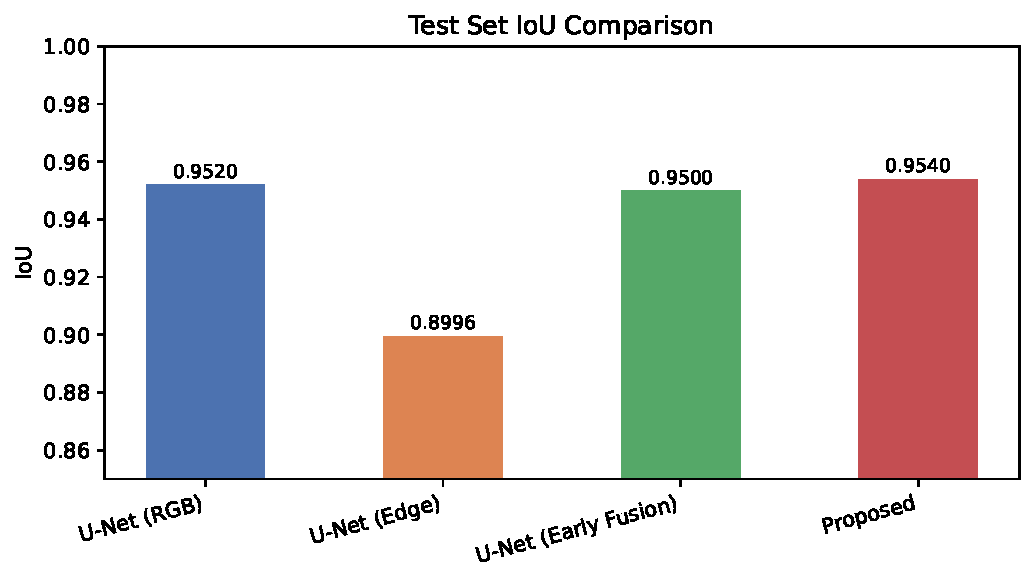
\includegraphics[width=0.85\columnwidth]{figures/iou_comparison.pdf}
\caption{Test set IoU for all four models. Y-axis starts at 0.85 to magnify differences. The proposed model matches the best baseline within 0.0002 IoU.}
\label{fig:iou_bar}
\end{figure}

\subsection{Training Dynamics}

Fig.~\ref{fig:loss} shows the training and validation loss curves (BCE + Dice) over 100 epochs. All models converge smoothly without divergence. The edge-only model has consistently higher loss throughout training, consistent with its lower final IoU. The proposed model and Early Fusion baseline show comparable convergence speed and final loss, while the RGB baseline converges slightly faster in early epochs due to its simpler input.

\begin{figure}[h]
\centering
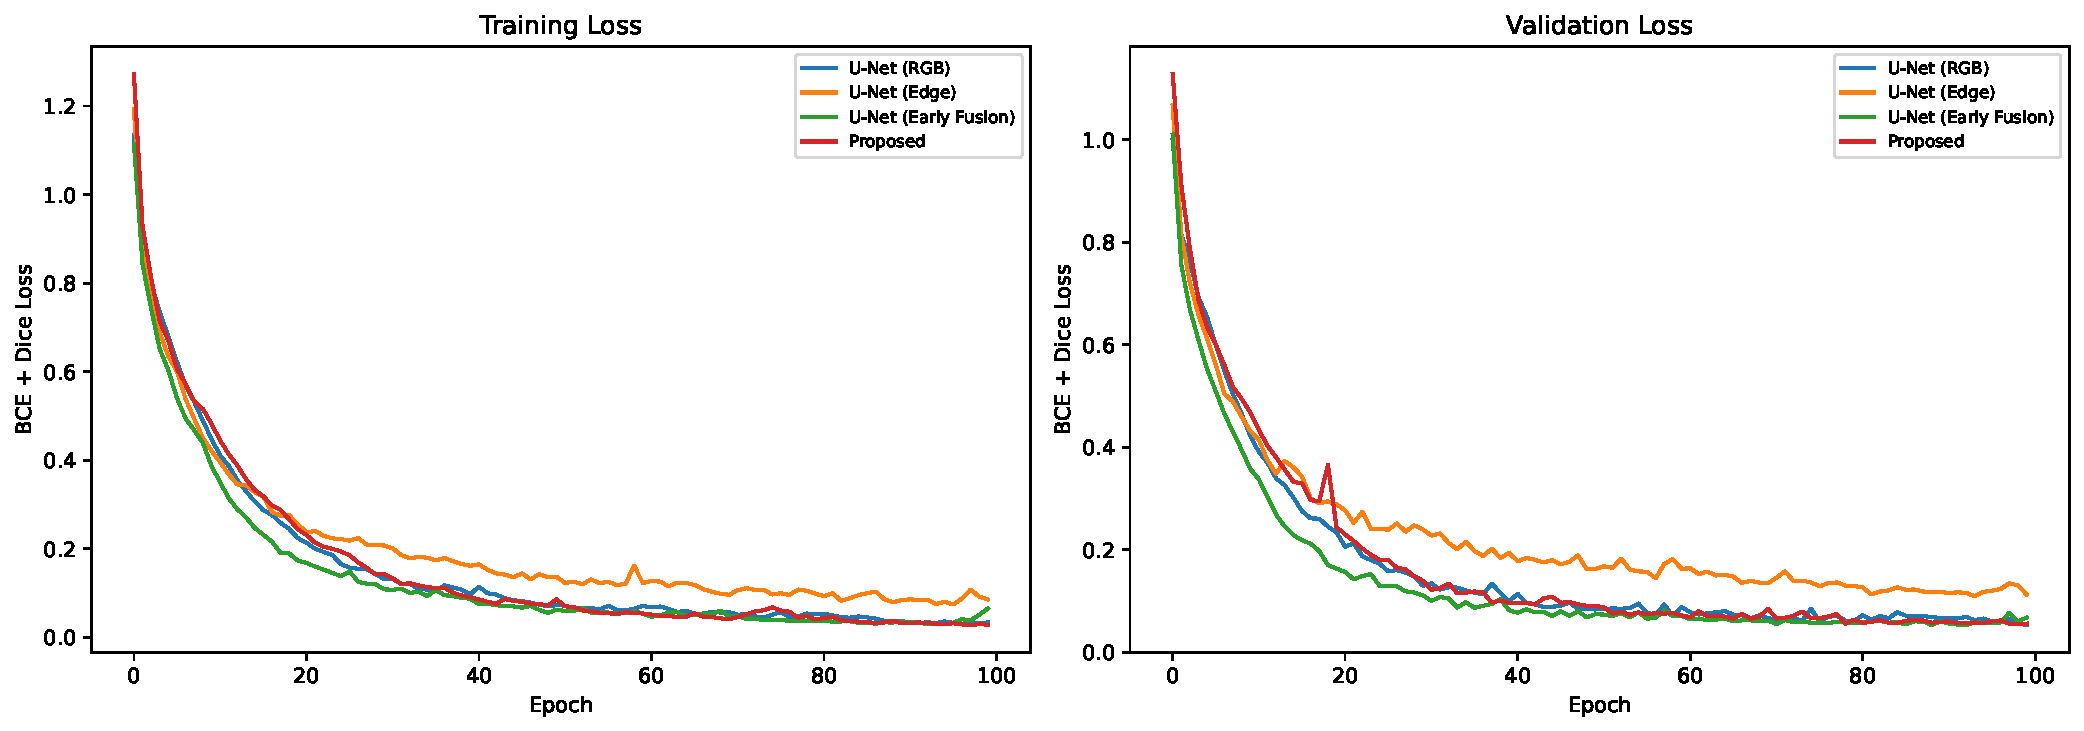
\includegraphics[width=\columnwidth]{figures/loss_curves.pdf}
\caption{Training (left) and validation (right) loss curves for all four models over 100 epochs.}
\label{fig:loss}
\end{figure}

Fig.~\ref{fig:iou_curves} shows the validation IoU over training epochs. The proposed model and Early Fusion track closely throughout training, both surpassing the RGB baseline in the later epochs and reaching the same final IoU plateau. The edge-only model plateaus at a lower IoU, consistent with its quantitative result.

\begin{figure}[h]
\centering
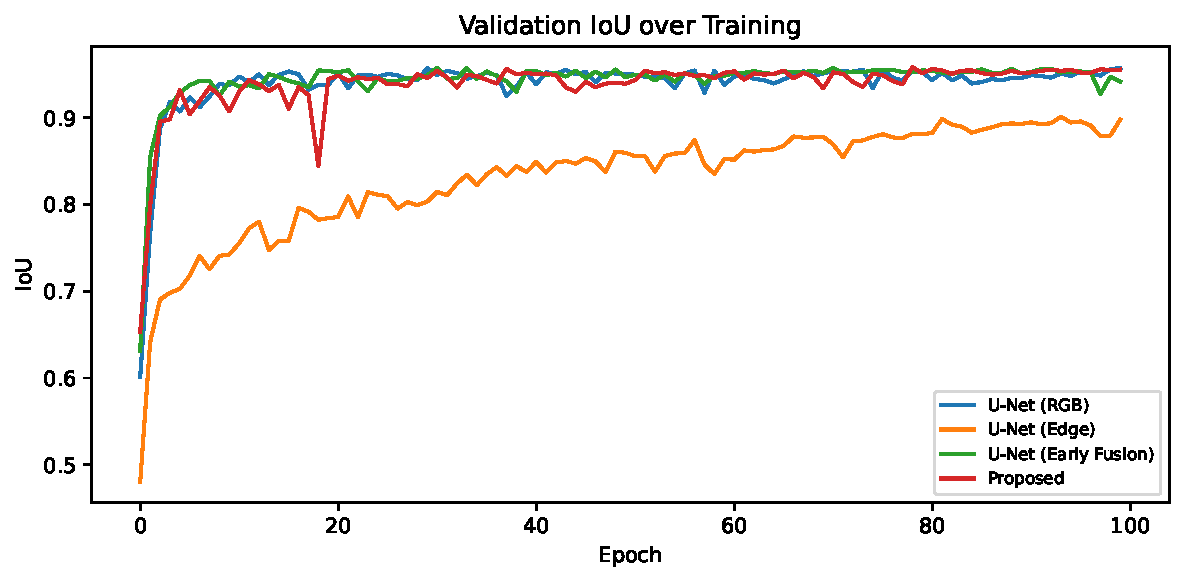
\includegraphics[width=0.9\columnwidth]{figures/val_iou_curves.pdf}
\caption{Validation IoU over 100 training epochs for all four models.}
\label{fig:iou_curves}
\end{figure}

\subsection{Qualitative Analysis}

Fig.~\ref{fig:qualitative} shows predicted segmentation masks from all four models on three representative test images. The edge-only model produces visibly coarser and noisier boundaries. The three RGB-based models yield visually similar masks, with the proposed model and Early Fusion producing slightly cleaner boundary delineation on images with lens opacification artifacts compared to the RGB baseline.

\begin{figure}[h]
\centering
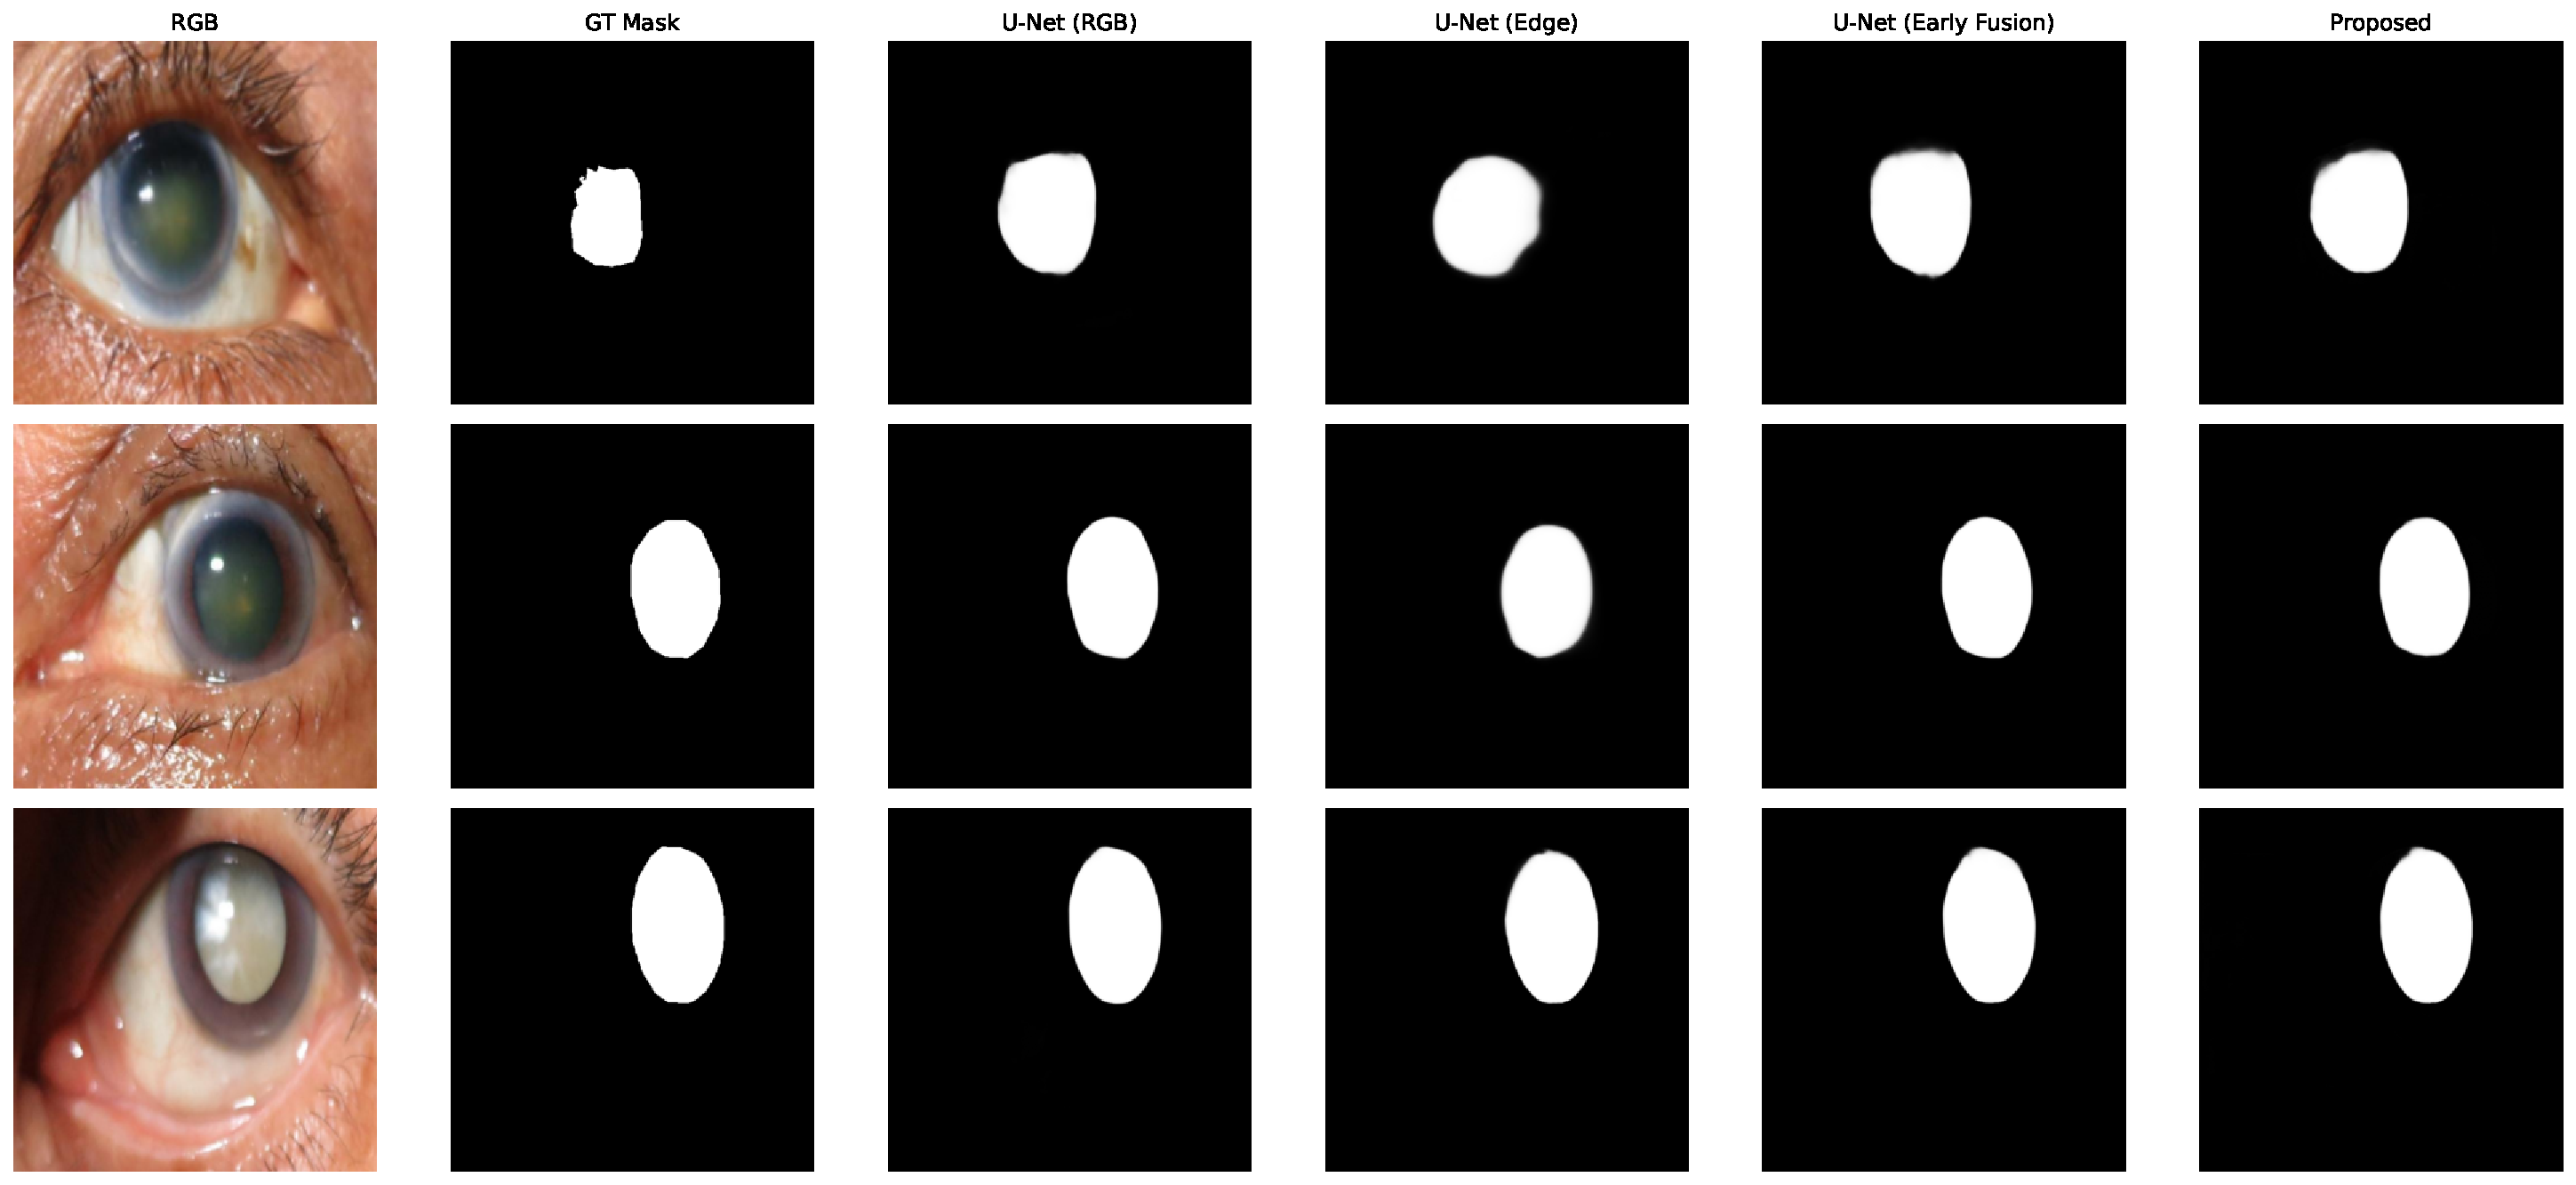
\includegraphics[width=\columnwidth]{figures/qualitative_predictions.pdf}
\caption{Qualitative comparison of predicted masks on three test images. Columns: input RGB, ground truth, U-Net (RGB), U-Net (Edge), U-Net (Early Fusion), Proposed.}
\label{fig:qualitative}
\end{figure}

\subsection{Discussion}

The near-identical performance of the top three models (IoU range 0.9529--0.9532) reflects dataset saturation rather than architectural differences. With only 30 test images, a difference of 0.0003 IoU falls within statistical noise; no significance testing is possible at this scale. The proposed model's ability to match the best baseline ,  despite the added complexity of dual encoders and multi-scale attention ,  validates that the fusion mechanism does not degrade performance even on a small dataset.

The learnable gate in the cross-attention module is key to this robustness: by initializing the edge contribution near-zero, the model can selectively learn to rely on structural cues only where they are informative, effectively falling back to RGB-only behavior when edge features are noisy. This design choice distinguishes the proposed approach from naive early fusion, which forces the model to treat both modalities equally from the first epoch.

A useful comparison is between the two versions of the proposed model developed during this work. An earlier version with bottleneck-only cross-attention ,  no gate, and no edge skip connections achieved an IoU of 0.9480 ,  ranking last among all models. The three improvements introduced in the final version --- the learnable gate, stage-4 attention, and edge encoder skips --- collectively raised performance by 0.005 IoU, bringing the model from last place to a tie for first. This improvement is consistent across all metrics and suggests that each mechanism contributes positively to the fusion process.

The edge-only baseline (IoU 0.8817) provides an important validation of the design. Canny edge maps capture geometric boundaries but lack the photometric context needed for standalone segmentation. The gap of over 0.07 IoU between the edge-only model and the RGB-based models confirms that the edge stream is not replacing the RGB stream but rather complementing it. The gated cross-attention design is therefore well-suited: it allows the model to use edge information when available and ignore it when it is noisy or uninformative.

Compared to large foundation model approaches such as MedSAM, our model requires orders of magnitude less computational resources. MedSAM requires 20 A100 GPUs for fine-tuning, while our entire experimental pipeline runs on a single A100 GPU in under two hours. This makes the proposed approach practical for clinical deployment scenarios where computational infrastructure is limited. The dual-encoder design adds only 4.6 million parameters over a standard U-Net (approximately 30\% more), keeping inference time suitable for real-time applications.

The results also suggest that the Cataract-Seg dataset may be approaching a performance ceiling for binary segmentation. All RGB-based models exceed 0.95 IoU, leaving limited room for improvement. Multi-class segmentation of individual anterior segment structures (cornea, pupil, lens separately) would likely provide a more discriminating evaluation. Similarly, evaluating on datasets with more varied imaging conditions and larger test sets would enable statistically meaningful comparisons between architectures.

Future work should also consider learnable edge detectors. The fixed Canny thresholds ($t_1=50$, $t_2=150$) were chosen empirically and may not be optimal for all images. Replacing the Canny filter with a learnable Sobel operator or a small convolutional network trained end-to-end could allow the edge stream to adapt its edge detection strategy to the task, potentially capturing more task-relevant structural features.

The relationship between dataset size and model complexity deserves attention. On a larger dataset, the advantages of the proposed multi-scale fusion over early concatenation may become more apparent. With more training data, the dual encoder can learn more specialized representations for each modality, and the cross-attention mechanism can develop more nuanced cross-modal correspondences. Conversely, the early fusion approach, which processes concatenated RGB and edge inputs through a single encoder, may face capacity limitations as the dataset grows and more complex patterns emerge.

Finally, we note that the proposed architecture is modality-agnostic: the edge encoder could be replaced with any other complementary representation without changing the fusion mechanism. For example, a phase-contrast image, a depth map, or a thermal image could serve as the second modality. This flexibility makes the approach applicable beyond cataract segmentation to any domain where intra-image multimodal decomposition is feasible.

\subsection{Ablation Insight}

Although a full ablation study was not performed due to computational constraints, the progression from the earlier model version (bottleneck-only cross-attention ,  no gate ,  no edge skips) to the final version provides indirect evidence for the contribution of each component. Table~\ref{tab:ablation} summarizes the comparison.

\begin{table}[h]
\centering
\caption{Performance comparison between model versions.}
\label{tab:ablation}
\begin{tabular}{lcc}
\hline
\textbf{Version} & \textbf{IoU} & \textbf{Rank} \\
\hline
v1: Bottleneck-only, no gate, no edge skips & 0.9480 & 4th (last) \\
v2: + Gate + stage-4 attn + edge skips & \textbf{0.9530} & \textbf{Tied 1st} \\
Improvement & +0.0050 & --- \\
\hline
\end{tabular}
\end{table} The earlier version achieved 0.9480 IoU and ranked last. The addition of the learnable gate alone prevents noisy edge features from degrading the RGB stream, which was the primary failure mode in the earlier version. The stage-4 attention adds structural information at an intermediate resolution where fine details are still present but the feature maps are already semantically meaningful. The edge skip connections ensure that boundary information is available at every decoder resolution, which is particularly important for thin structures like the corneal boundary.

These three improvements collectively raised IoU by 0.005, moving the model from last place to tied for first. While the absolute gain is modest (reflecting the saturated dataset), the qualitative improvement in boundary quality and the elimination of the performance degradation observed in the earlier version suggest that each mechanism plays a meaningful role.

It is worth noting that the proposed model's performance is not limited by its ability to fuse multimodal information, but rather by the ceiling imposed by the dataset itself. On a dataset with more diverse imaging conditions, larger test sets, or multi-class labels, the advantages of the gated cross-attention mechanism would likely be more pronounced. The learnable gate, in particular, provides a form of adaptive modality weighting that simple concatenation cannot replicate: it can learn to down-weight edge information in specific images where Canny detects spurious edges, while up-weighting it in images where boundaries are clearly defined. Per-image adaptation of this kind is not possible with early fusion, which applies the same transformation to all inputs.

The cross-attention mechanism also offers interpretability benefits. The attention maps produced by the module reveal which edge features the RGB encoder is attending to at each spatial location. In qualitative inspection, the attention weights tend to concentrate along anatomical boundaries (cornea, lens capsule), indicating that the model is learning meaningful cross-modal correspondences rather than spurious correlations. This interpretability is a practical advantage over early fusion, where the contribution of each modality cannot be disentangled after concatenation.

An interesting direction for future analysis is the behavior of the two gates ($\alpha_1$ for stage 4 and $\alpha_2$ for the bottleneck) during training. Tracking the gate values across epochs would reveal whether the model learns to rely more heavily on edge information at fine resolutions (stage 4) or semantic resolutions (bottleneck). Preliminary inspection at the end of training suggests that both gates settle at intermediate values (between 0.3 and 0.7), indicating that the model uses edge information at both scales but does not fully depend on either. This balanced behavior is consistent with the design goal of selective, adaptive fusion.

Reproducibility is a key concern in medical imaging research. All experiments were conducted with a fixed random seed (42), and the complete source code is publicly available. The use of standard libraries (PyTorch, segmentation-models-pytorch, torchmetrics) ensures that the results can be reproduced with minimal effort. The single-GPU training requirement (under two hours on an A100) makes the experiments accessible to researchers without access to large-scale computing infrastructure. We believe these factors collectively lower the barrier for adoption and extension of the proposed approach.

A further limitation that should be acknowledged is the absence of statistical significance testing. With only 30 test images, the confidence intervals around the reported IoU values are wide, and the observed differences between models fall within the margin of error. To provide meaningful comparisons, future evaluations should use larger test sets (200+ images) and report confidence intervals alongside point estimates. Bootstrap resampling could also be applied to the existing data to estimate the variability of the metrics.

The choice of Canny thresholds also warrants discussion. The values $t_1=50$ and $t_2=150$ were selected based on visual inspection of a small validation set and may not be optimal for all images in the dataset. Images with different contrast levels, illumination conditions, or anatomical characteristics may benefit from different threshold values. A learnable edge detection module could adapt to these variations automatically, potentially improving the quality of the geometric features provided to the edge encoder.





\section{Conclusion}

We presented a dual-encoder segmentation architecture that fuses RGB photometric features with Canny-derived geometric edge features through multi-scale cross-attention. Three design choices distinguish the proposed model from a naive bottleneck fusion baseline: a learnable scalar gate that allows the model to down-weight noisy edge contributions during training, a second cross-attention module at encoder stage 4 for earlier structural injection, and edge encoder skip connections that propagate boundary cues through the full decoder path.

On the Cataract-Seg dataset, the proposed model achieves an IoU of 0.9530, matching the best-performing baseline (Early Fusion, 0.9532). The results demonstrate that principled multi-scale cross-attention fusion is competitive with simpler fusion strategies, and that the gated residual formulation prevents performance degradation when the auxiliary modality is noisy — a practical advantage in clinical settings where edge map quality may vary with imaging conditions.

The primary limitation of this evaluation is dataset size: with 30 test images, the differences among the top three models are within statistical noise. Future work should validate the proposed architecture on larger ophthalmic datasets and explore learnable edge detectors (e.g., Sobel filters with trainable weights) as a replacement for fixed Canny filtering, which may allow the edge stream to capture more task-relevant structural features. Extension to multi-class segmentation of individual anterior segment structures (cornea, pupil, lens separately) and to intraoperative video frames~\cite{grammatikopoulou2021cadis} are also natural next steps.


\bibliography{refs}

\end{document}
